\documentclass{beamer}

\usepackage{graphicx}
\usepackage[english]{babel}

\hypersetup{pdfstartview={Fit}}
\setbeamertemplate{navigation symbols}{}

\begin{document}

\title[LOD] % (optional, only for long titles)
{Linked Open Data at Universities}
\subtitle{A case study concerning students}
\author[Author, Haller] % (optional, for multiple authors)
{Kevin Haller}

\date[2016] % (optional)
{Seminar Work, 2016}
\subject{Computer Science}

\frame{\titlepage}

\begin{frame}
\frametitle{Table of Contents}
\tableofcontents[hideallsubsections]
\end{frame}


\begin{frame}
\section[Introduction]{Introduction}
\frametitle{Introduction}
\end{frame}

% --------------------------------------------------------------------------------------------
%  Result: Case study
% --------------------------------------------------------------------------------------------

\begin{frame}
\section[Benefits and challenges]{Benefits and challenges of using Linked Open Data at universities}
\frametitle{Benefits and challenges}

\end{frame}

\begin{frame}
\subsection[Interviewees background]{Interviewees background}
\frametitle{Interviewees background}
\begin{table}[h]
	\small
	\begin{tabular}{| l | c | c | c | c |}
 		\multicolumn{2}{c|}{} & \multicolumn{2}{c|}{Level of expertise} \\
 		\hline
		ID & Assignment & ICT (1-5) & LOD (1-5) & Date of interview \\
		\hline
		A  & student representative & 3 & 1 & 24.11.2015\\
		B & teaching \& administration & 5 & 2 & 03.12.2015\\
		C & teaching \& administration & 5 & 1 & 17.12.2015\\
		D & student & 4 & 3 & 12.02.2016\\
		E & student & 4 & 3 & 18.02.2016\\
		\hline
	\end{tabular}
	\label{table:interviewee-background}
\end{table}
\begin{block}{Scala for level of expertise}
\begin{table}[h]
	\footnotesize 
	\begin{tabular}{ c | l  | p{6.5cm} }
		Value & ICT & LOD\\	
		\hline
		1 & Fundamental & I never heard of Linked Open Data.\\
		\hline
		2 & Novice & I heard of Linked Open Data, but never used it.\\
		\hline
		3 & Intermediate & I used Linked Open Data in a not intense way. E.g. as part of a workshop or home project.\\
		\hline
		4 & Advanced & I used Linked Open Data in a practical project.\\
		\hline
		5 & Expert & I used Linked Open Data in several practical projects and consider myself an expert in Linked Open Data.\\
	\end{tabular}
	\label{table:interviews-rating scales}
\end{table}
\end{block}
\end{frame}


% --------------------------------------------------------------------------------------------
%  Result: Technical architecture and challenges
% --------------------------------------------------------------------------------------------

\section[Technical architecture and challenges]{Technical architecture and challenges}
\begin{frame}
\subsection{Linked Open Data effort at universities}
\frametitle{Linked Open Data effort at universities}
	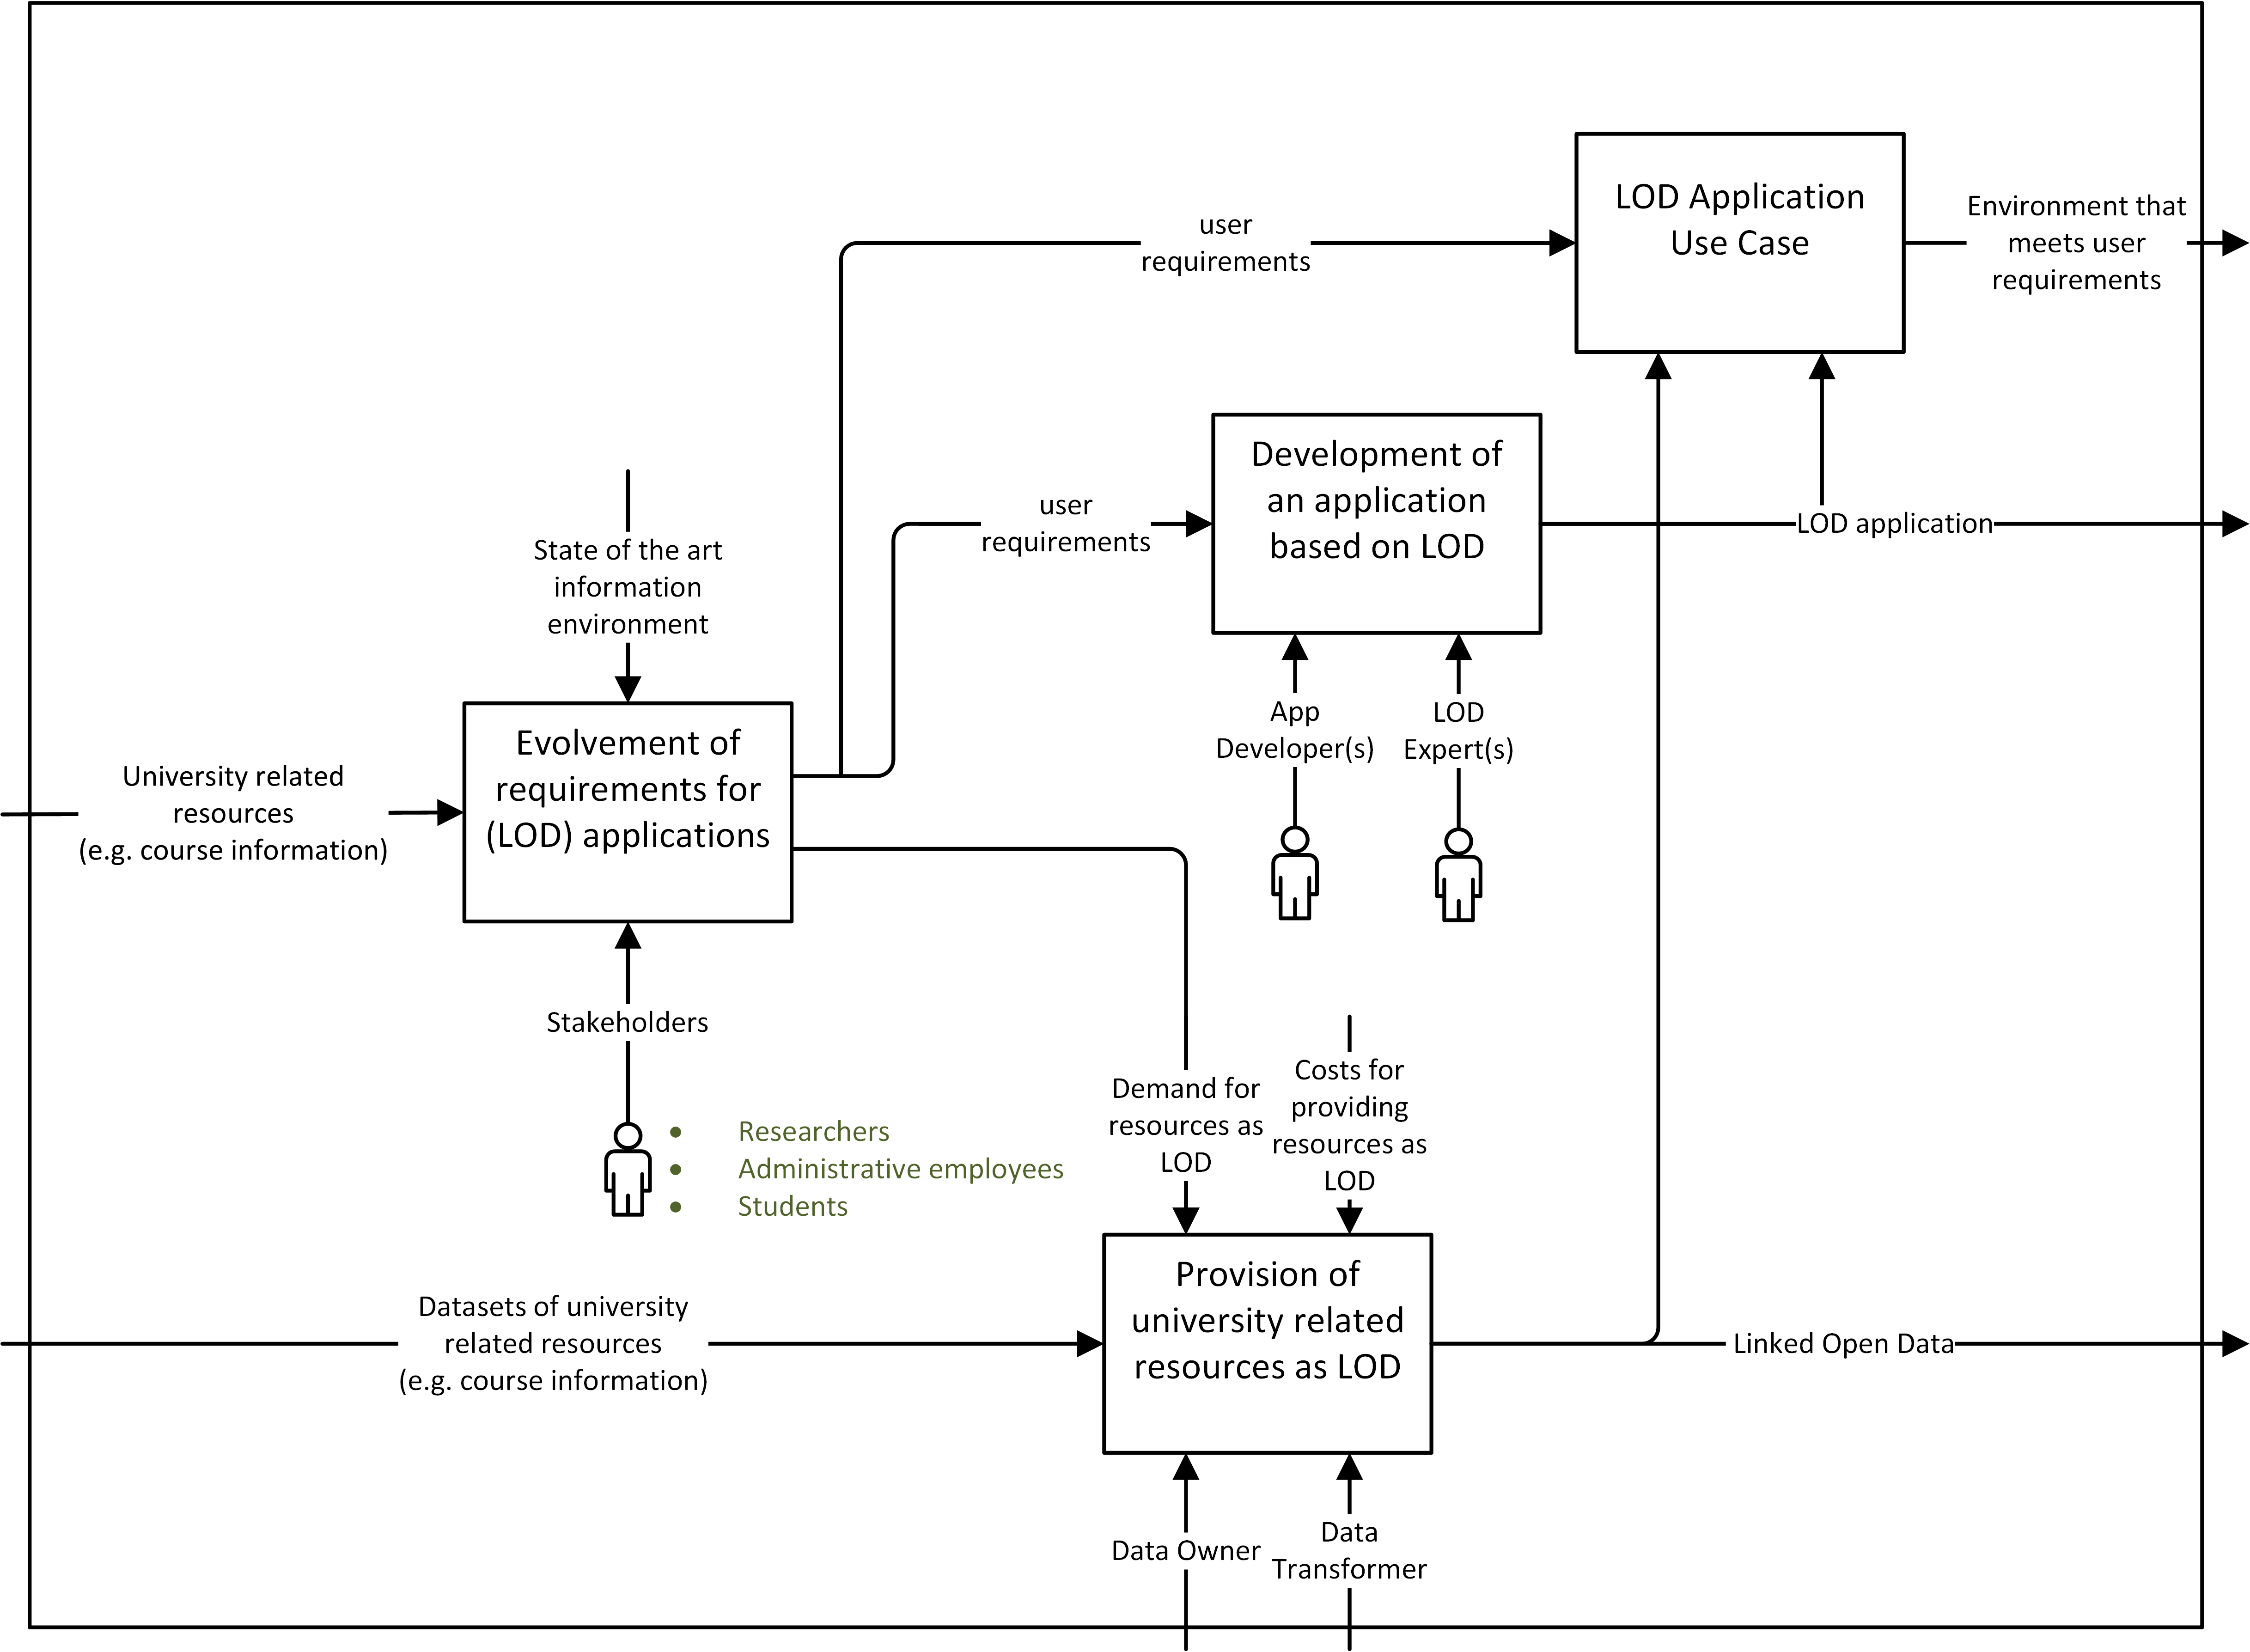
\includegraphics[width=\columnwidth]{../images/technical-architecture/lod_at_tuwien_idef0.png}
\end{frame}
\begin{frame}
\subsection{Proposal of technical architecture}
\frametitle{Proposal of technical architecture}
	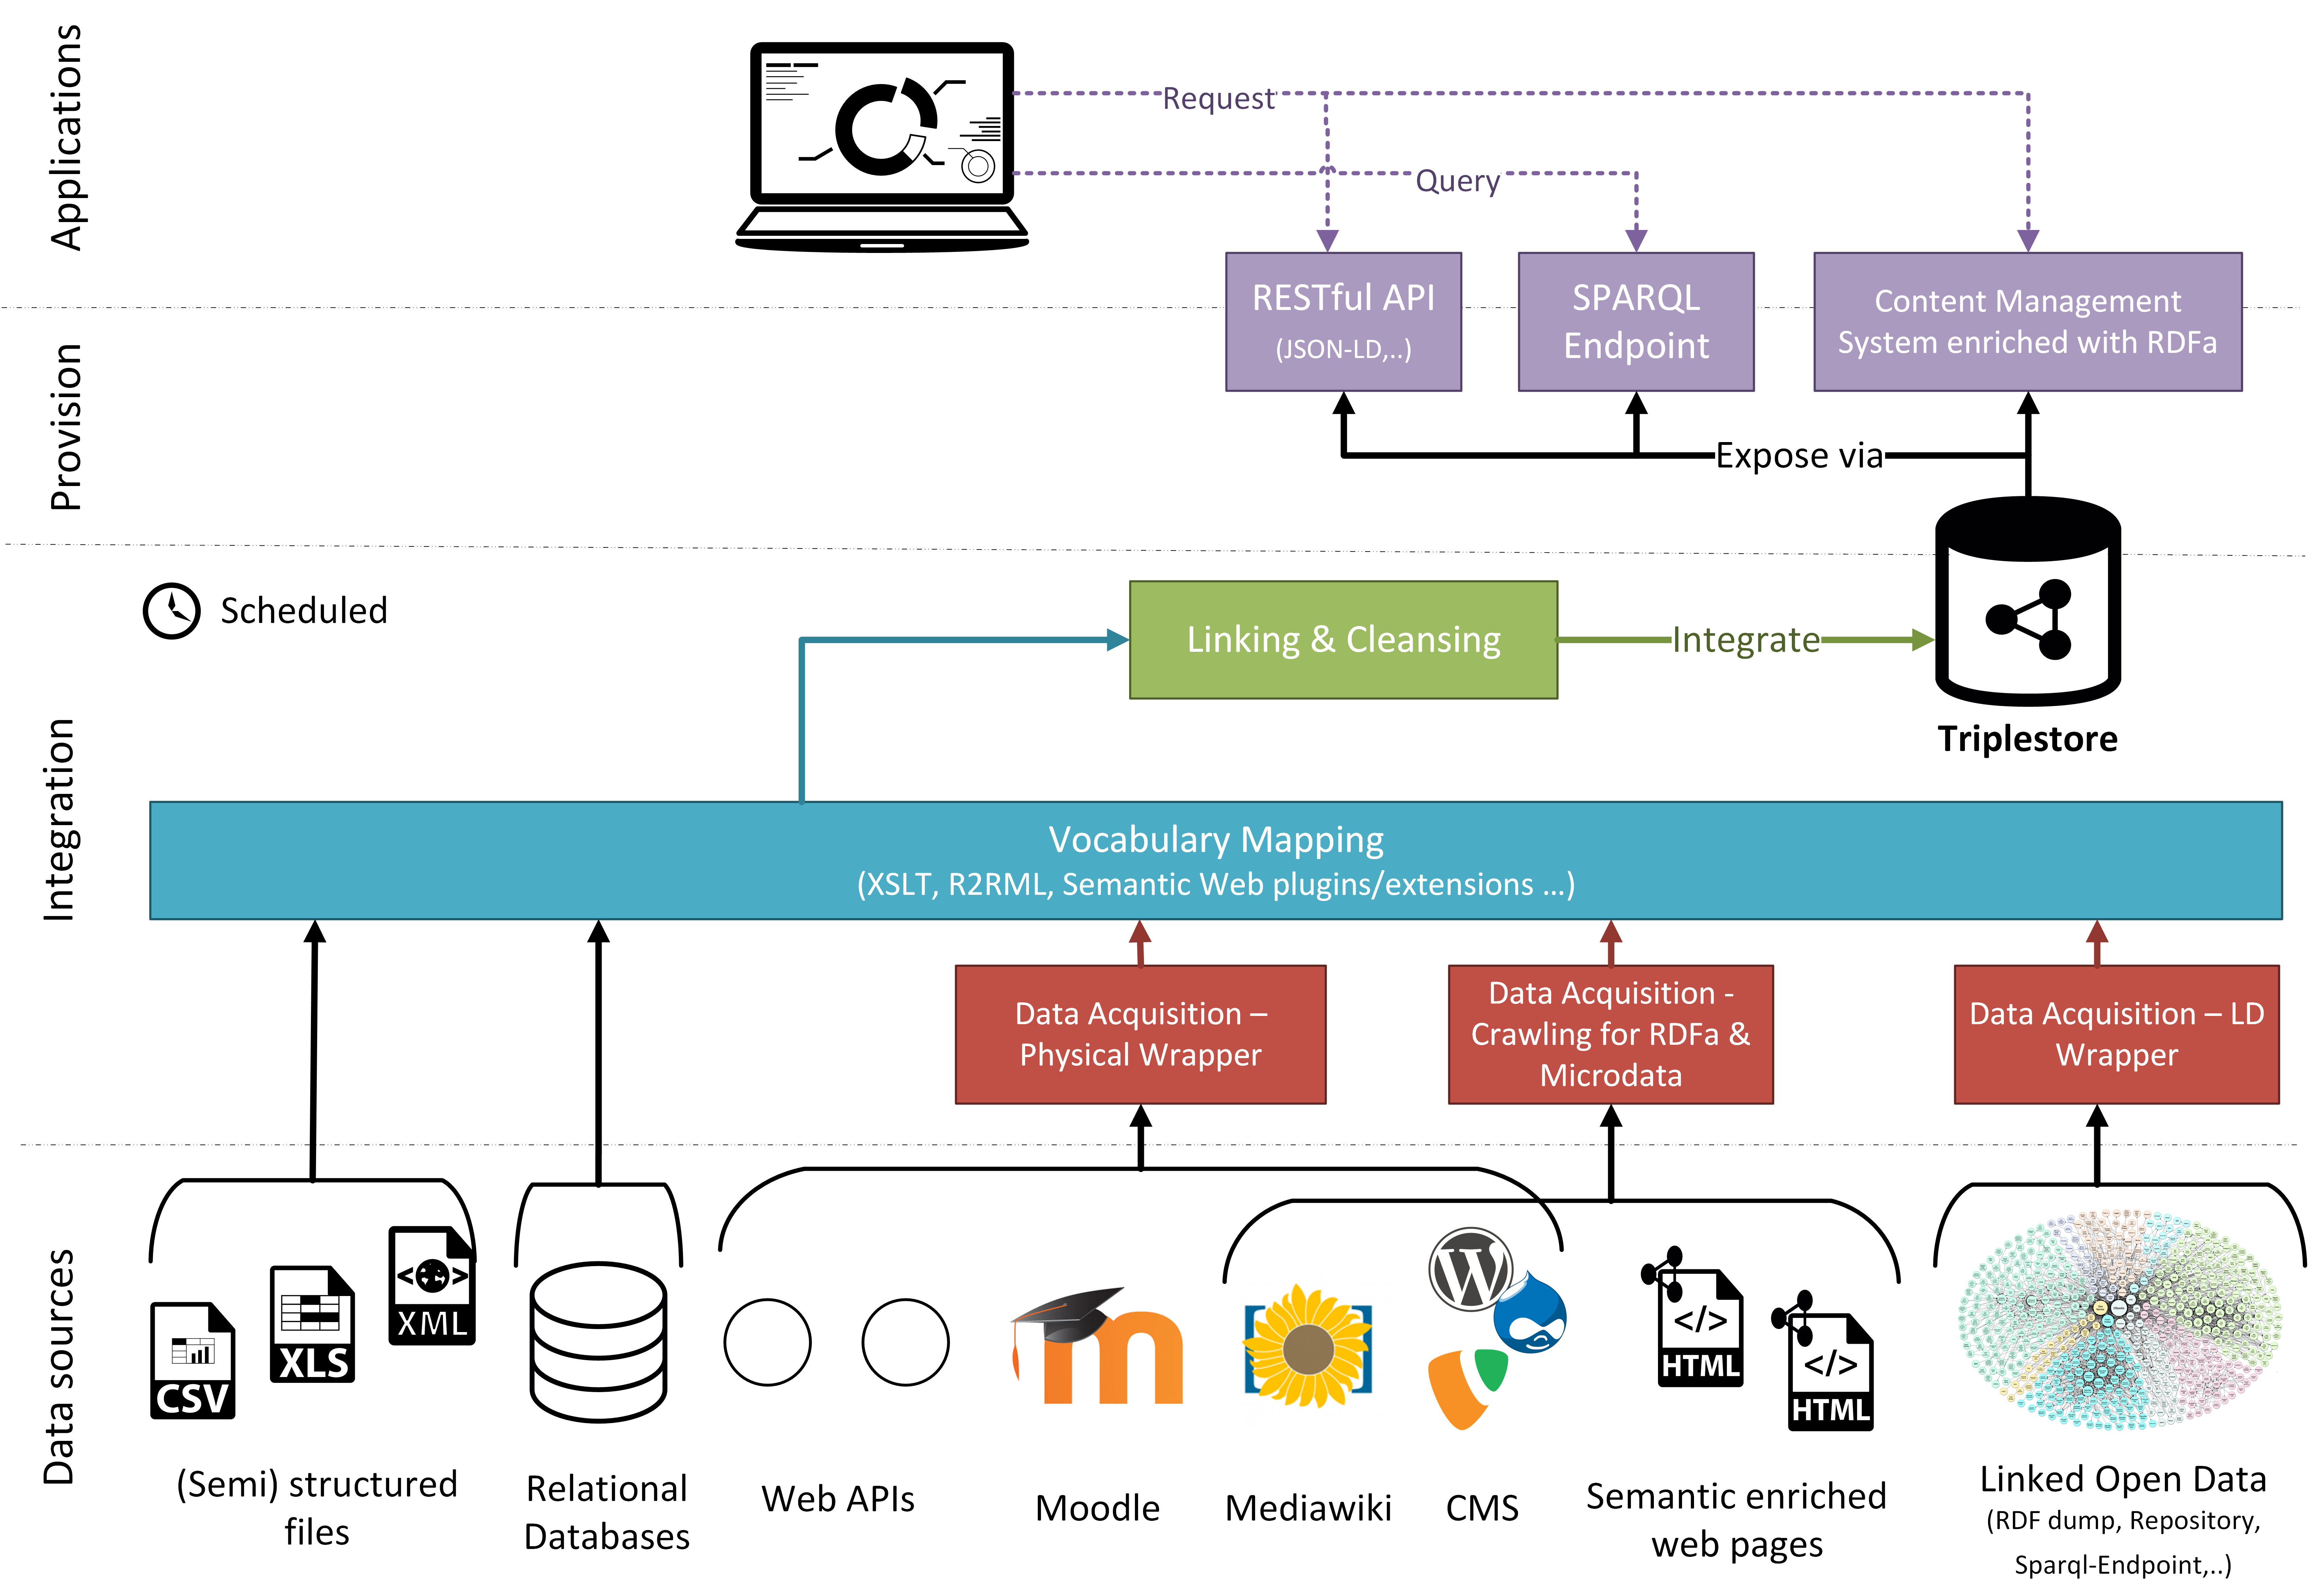
\includegraphics[width=\columnwidth]{../images/technical-architecture/lod_technical_architecture.png}
\end{frame}

\subsection{Challenges}
\begin{frame}
\frametitle{Challenges}
\end{frame}

\subsubsection{Data ownership}
\begin{frame}
\frametitle{Challenges}
\framesubtitle{Data ownership}
\end{frame}

\subsubsection{Data licenses}
\begin{frame}
\frametitle{Challenges}
\framesubtitle{Data ownership}
\end{frame}

\subsubsection{Data freshness}
\begin{frame}
\frametitle{Challenges}
\framesubtitle{Data ownership}
\end{frame}

\end{document}